\documentclass{bioinfo}
%\documentclass{article}
\input{logicmacros}
\usepackage{url}


\ifx\pdfoutput\undefined
% we are running LaTeX, not pdflatex
\usepackage{graphicx}
\else
% we are running pdflatex, so convert .eps files to .pdf
%\usepackage[pdftex]{graphicx}
%\usepackage{epstopdf}
\fi 

\copyrightyear{}
\pubyear{}

\def\P1{\pr{P-1}}

\def\partOfT{\pr{part\_of$^T$}}
\def\partOf{\pr{part\_of}}
\def\hasPart{\pr{has\_part}}
\def\isA{\pr{is\_a}}
\def\instanceOf{\pr{instance\_of}}
\def\derivesFrom{\pr{derives\_from}}
\def\adjacentTo{\pr{adjacent\_to}}

\def\existsAt{\pr{exists\_at}}

\def\partOfAtSomeTimes{\pr{part-of-at-some-times}}
\def\partOfAtAllTimes{\pr{part-of-at-all-times}}
\def\hasPartAtSomeTimes{\pr{has-part-at-some-times}}
\def\hasPartAtAllTimes{\pr{has-part-at-all-times}}
\def\hasPartAtAllTimesForWhichPartExists{\pr{has-part-} \pr{at-all-times-}\ \pr{for-which-part-exists}}
\def\partOfAtAllTimesForWhichWholeExists{\pr{part-of-} \pr{at-all-times-}\ \pr{for-which-whole-exists}}

\def\atAllTimes{\pr{at-all-times}}
\def\atSomeTimes{\pr{at-some-times}}
\def\atAllTimesForWhichPartnerExists{\pr{at-all-times-for-which-partner-exists}}

\def\CellNucleus{\pr{cell nucleus}}
\def\Cell{\pr{cell}}

\def\OBOREL{\textbf{OBO-REL}}

\newcommand{\tbleqn}[1]{
\begin{math}
\begin{aligned}[1]
#1
\end{aligned}
\end{math}
}

\begin{document}
\firstpage{1}

\title{A critique of temporalized relations}

\author{Christopher J. Mungall\,$^{1}$\footnote{to whom correspondence should be addressed}}
\address{$^{1}$Genomics Division, Lawrence Berkeley National Laboratory, MS84R017, 1 Cyclotron Road, Berkeley, CA 94720 USA}

\history{}

\editor{}

\maketitle

\begin{abstract}

  In this review I evaluate the proposed new temporalized relations
  strategy in which many existing relations would be replaced by two
  or more relations, an \emph{at-all-times}\ form and an
  \emph{at-some-times}\ form.

  My findings are that the \emph{at-all-times}\ relations have an
  underlying logical problem that renders them formally incorrect for
  use in many ontologies. The \emph{at-some-times} relations are
  safer, but would lose crucial transitive inferences. These logical
  problems are compounded by the fact that the relations are difficult
  for users and ontology developers to understand, and will most
  likely lead to confusion and errors, especially in the absence of
  detailed documentation and extensive training.

  I conclude that these relations should not be adopted by ontology
  developers as a replacement for existing atemporal
  relations. Migrating to these relations would be an expensive,
  error-prone process that would confuse and alienate users; the end
  result would be ontologies that are either formally incorrect or too
  weak to derive required inferences.

\end{abstract}

\section{Introduction}

\subsection{The OBO Relations ontology}


The OBO relations ontology (\OBOREL) defined a set of core relations
for use in biological ontologies, including \isA, \partOf\ and
\derivesFrom\cite{Smith2005}. The original \OBOREL\ paper has been
cited 709 times\footnote{Google scholar}, and has been a crucial
reference in the correct usage of relations in biological ontologies.

One notable aspect of \OBOREL\ was the precise specifications of how
relationships change or remain the same through the passage of
time. For example, the intent was that an ontology would state that
\emph{every} \CellNucleus\ is part of \emph{some} \Cell\ at \emph{any}
given moment of time (for which the given cell nucleus exists). This
statement has a precise formulation in first-order logic (FOL):

$
\A x \A t : \instanceOf(x, \CellNucleus, t) \imp \\
 \E y \instanceOf(y, \Cell, t), \partOf(x,y,t)
$

%A relationship of this form is known as \emph{permanent generic
%  parthood}. It allows for nuclei to be passed from one cell to
%another, so long as the nucleus remains part of some cell. 

The other notable aspect of \OBOREL\ was the distinction between type
(class) -level and instance -level relations. Each type-level relation
connects a pair of classes and serves as a shorthand for writing
complete FOL axioms. For example, writing $\CellNucleus\ \partOfT\
\Cell$ is equivalent to writing the full FOL axiom above. (Note that
in contrast to the original paper, I denote type-level relations via
a $^T$ superscript).

\subsection{OBO-REL and OWL}

\OBOREL\ initially served as the foundational semantics for many
ontologies in the OBO library\cite{Smith2007}. However, with the
decision to define OBO-Format in terms of the Web Ontology Language
(OWL)\cite{golbreich2007obo,OBOFormat}, the role of the \OBOREL\
interpretation became unclear. To see why, consider a typical OWL
axiom from the Gene Ontology\cite{Ashburner2000}:

\begin{verbatim}
'cell nucleus' SubClassOf part_of some cell
\end{verbatim}

The \partOf\ relation (or Object Property, in OWL terminology) used
here is not the same as the ternary time-indexed instance relation
from \OBOREL, neither is it the same as the type-level
counterpart. The semantics of the OWL axiom are atemporal, and
translate to:

$
\A x : \instanceOf(x, \CellNucleus) \imp \\
 \E y \instanceOf(y, \Cell), \partOf(x,y)
$

This is clearly different to what is specified in the \OBOREL\ paper.
In practice, the developers of ontologies subscribe nominally to the
\OBOREL\ interpretation but use binary atemporal OWL object properties
from the new version of the OBO Relations Ontology\cite{RO2010}.

Assessing the negative impact of this interpretation mismatch is not
straightforward. For most practical purposes it has not caused any
problems, but there are concerns regarding interoperability and how to
use ontologies in combination with instance data. There are ongoing
efforts to align these interpretations, but I do not discuss them here
- instead I focus on a proposal that does away with these atemporal
relations, and replaces them with explicitly temporalized relations,
coupled to the release of BFO2.

\subsection{BFO2 and temporalized relations}

The Basic Formal Ontology (BFO) is an upper level ontology intended
for use in the sciences\cite{Grenon2004}. Version 2 of BFO (BFO2)
comprises two components: (1) the BFO2 \emph{reference}\cite{BFO2Ref}
which is specified independently of OWL, and (2) the OWL realization
of this reference. The reference is specified using FOL and uses
ternary time-indexed relations akin to the instance-level relations of
the original \OBOREL\ paper. One of the goals of the group developing
the OWL version was to have relations in OWL handled so as to have a
clear First-Order Logic (FOL) reading according to the BFO
reference. This is enshrined in principle number 1 (called \P1\ from
here on) from the BFO
wiki\footnote{http://code.google.com/p/bfo/wiki/
  Proposal\_for\_how\_we\_manage\_OWL\_Reference\_coordination}:

\begin{quotation}
  \emph{A clear reading of the OWL version in terms of BFO reference. A
  translation is a mapping from the OWL model - axioms, entities,
  relations, etc. To the formal language used in the reference,
  currently FOL. A reading can be considered a data transformation
  that takes asserted and inferred axioms and results in FOL using
  types defined in BFO2 reference. This translation should be complete
  - no assertions in the OWL file can be left untranslated. In our
  current version, the most obvious missing reading is of binary
  relations with the same name as the ternary time-indexed relations
  in BFO2 reference}.
\end{quotation}

The BFO group explored different approaches for modeling relations in
OWL in a way that is conformant with \P1. One strategy involves
retaining retaining simple atemporal binary properties in the OWL, and
adhering to \P1\ by means of different or additional interpretations
of the OWL semantics\cite{Grewe}. This can be considered a kind of
``default strategy''.  Another approach involves treating ontologies
as capturing ``snapshots'', so-called \emph{Temporally Qualified
  Continuants}. In this document, I do not consider these
alternatives, and I focus solely on the \emph{temporalized relations}
(TR) approach, in which each ternary time-indexed relation has two or
more OWL ObjectProperty cognates, \pr{rel-at-some-times} and
\pr{rel-at-all-times}. This approach was used to create the BFO2 OWL
Graz release\cite{Graz}, which is intended to be the basis of the
final version of BFO2.

This approach has proven unpopular with ontology developers and users
of ontologies largely due to confusion over the proliferation of
relationship types\cite{BFO2InformalSurvey}. In this critique I
demonstrate that the problems with this approach run deeper than mere
profusion of relations, and that this approach has severe negative
impact for both short and long term use in OWL ontologies.

\subsection{Outline}

In this critique I focus solely on the temporalized relations
approach. I do not attempt to compare or even describe the different
modeling possibilities (see \cite{Grewe} for details here).

In section 2 I provide an outline of temporalized relations, drawing on
the existing release notes and documentation, attempting to fill some
gaps and provide additional explanations of some of the
complexities. Then in section 3 I present the major problems posed by
these relations:

\begin{enumerate}

\item \textbf{logic issues}: Many problems arise from the logical
  underpinnings of the temporalized relations approach. The semantics
  of these relations cannot be expressed in OWL, limiting our ability
  to use OWL reasoners. Furthermore, the semantics of these relations
  are different from those intended by ontology developers, leading to
  ontologies that are either formally not valid or incomplete.

\item \textbf{usability issues}: Temporalized relations would lead to
  an unacceptable increase in complexity in most ontologies.

\end{enumerate}

These problems are inter-related; the complexity of the approach with
its proliferation of unintuitive relations masks underlying logical
problems. Ontology editors who do not understand the formalism are
more likely to make errors, both in migrating to temporalized
relations, and in maintaining ontologies that use them.

After illustrating these logical and usability problems, I end with
some concrete recommendations regarding the temporalized relation
strategy (section 4).

My intentions are to make this review accessible to a wide audience,
and to keep logical formulas to a minimum. This is difficult because
to understand the motivations of the TR approach and the underlying
problems it is necessary to understand some of the logical
underpinnings. I have annexed some of the finer grained details into
an appendix, and attempted to stick with examples a biologist would
understand.

\begin{table}
\begin{tabular}{ | p{2.5cm} | p{1cm} | p{1cm} | p{2cm} | }
\hline
\textbf{Object Property} & \textbf{Trans} & \textbf{Symm} & \textbf{Inverse Of}  \\
\hline
\partOf\  & Yes & No & \hasPart  \\
\hline
\hasPart\ & Yes & No & \partOf \\
\hline
\adjacentTo\ & No & Yes &  \\
\hline
\end{tabular}
\caption{Relation characteristics, atemporal. These are the characteristics of the instance level relations in the current RO (http://obo-relations.googlecode.com)}
\label{tab:characteristics-atemporal}
\end{table}

\section{Temporalized Relations}

\subsection{Preliminary definitions}

To avoid confusion, it is necessary to be clear about the different
forms and interpretations of relations.

\begin{enumerate}

\item \emph{Reference Relations} (RRs) include instance-level
  relations specified in the BFO2 reference. An example is the
  continuant version of the \partOf\ relation. For space reasons I
  focus solely on ternary time-indexed RRs in this critique. These
  relations cannot be directly expressed in OWL.

\item \emph{Temporalized Relations} (TRs) are OWL object properties
  that correspond to an RR combined with a temporal qualifier. An
  example is \partOfAtAllTimes. As these are OWL object properties,
  they are necessarily binary and instance-level.

\item \emph{Class-level Relations} (CLRs) are binary relations that
  hold between classes, as specified in the original \OBOREL\ paper. I
  focus neither on these relations nor on difficulties representing
  these in OWL, but sometimes it is necessary to mention these to
  shown comparisons with the original OBOREL paper.

\item \emph{Atemporal Relations} (ARs) are OWL object properties that
  are typically in one-to-one correspondence with RRs, but are not
  explicitly temporalized. As these are OWL object properties, they
  are necessarily binary and instance-level. Table
  \ref{tab:characteristics-atemporal} shows some example ARs and their
  characteristics. At this time, ARs lack a defined, agreed upon
  temporal reading (i.e. a mapping to FOL that introduces the temporal
  argument), which motivates the replacement of ARs with TRs in the
  current BFO2 proposal.

\end{enumerate}

As a typographical convention, I use dashes to separate words in a TR
(e.g. \partOfAtAllTimes). Underscores are used to separate the words
in a RR or AR (e.g. \partOf). RRs and ARs are disambiguated by their
context - OWL axioms use ARs and 3-argument FOL sentences use RRs.

On the occasions where CLRs are used, a $^T$ is suffixed onto the
relation name (e.g. \partOfT).


\subsection{Translation template}

The BFO2 Graz version release notes\cite{Graz} specify a general
template for relating RRs to TRs:

\begin{verbatim}
x rel-at-some-time y ->
 exists(t) exists_at(x,t) -> 
    exists_at(y,t) and rel(x,y,t)
x rel-at-all-times y ->
  forall(t)  exists_at(x,t) -> 
      exists_at(y,t) and rel(x,y,t)
\end{verbatim}

I interpret this as macro-expansion rules\footnote{Awaiting confirmation -
see http://code.google.com/p/bfo/issues/detail?id=154}.

Here I focus on \partOf\ as an exemplar relation, whilst recognizing
that similar patterns may apply to other, but not all relations.

For \partOf\ connecting two continuants there are in fact \emph{three}
TRs rather than two (for reasons that will be explained shortly):

\begin{enumerate}

\item \partOfAtSomeTimes

\item \partOfAtAllTimes

\item \partOfAtAllTimesForWhichWholeExists

\end{enumerate}

Note that in BFO2 the actual labels are ``part of continuant at some
time'', ``part of continuant at all times'' and ``part of continuant
at all times for which whole exists'', I shorten this for brevity --
here we are only concerned with relations that involve a continuant.

\subsection{TRs do not mean the same thing as OBOREL}

On the surface, the \atAllTimes\ form appears to be the same as the
\OBOREL\ interpretation. For example, an ontology that uses TRs may
include the following OWL axiom:

\begin{verbatim}
'cell nucleus' SubClassOf
   part-of-at-all-times some cell
\end{verbatim}

This may seem to be the same as the OBOREL statement
$\CellNucleus\ \partOfT\ \Cell$. If it were, this would be very
convenient - we could simply use \partOfAtAllTimes\ every time an
ontology author intended the \OBOREL\ interpretation, facilitating
automatic translation of an ontology to a TR form.

\emph{However, these are NOT the same, and an understanding of why
  this is so is crucial if these relations are to be used correctly,
  and to understand the long-term consequences of adopting the TR
  strategy}.

It is not the case that TRs are the same as what has come before, but
with longer labels. \emph{The semantics are fundamentally different}.
This has major effects on both the OWL axioms that are crucial for
reasoning over ontologies, and on the FOL reading of what the axioms
in the ontology means. See \textbf{table \ref{tab:fol-class-axioms}}
in the appendix to compare the FOL for TRs vs \OBOREL. For readers not
versed in FOL, I will next provide an outline of how the TR semantics
affect the OWL \emph{characteristics} of these relations in some ways
that might seem surprising. I will return to this in the evaluation to
show how this affects real-world ontology modeling.

\subsection{Object property characteristics}

In OWL, relations (object properties) can have certain characteristics
such as being \emph{transitive}, \emph{symmetrical}, and they may be
related to other relations via logical axioms such as \emph{inverse
  properties} and property chains. These are extremely useful for many
purposes - transitivity has been at the core of bioinformatics
applications of ontologies from the initial version of the Gene
Ontology\cite{Ashburner2000}, if not before. Inverse properties are
useful for instance level reasoning, and for finding errors in complex
ontologies.

When translating a RR to a TR, it may not be immediately clear what
properties of the RR should be carried over to the TR. If a reference
relation $R$ has an inverse $R'$, \emph{it does not follow that the
temporalized versions will be inverses}. Here I use \partOf\ as an
illustrative example, although each relation may require individual
examination for its properties.

Figure \ref{fig:part} shows the characteristics of continuant parthood
relations, both atemporal (A) and temporalized (B).

%----------------------------------------
\begin{figure}
\center
\includegraphics[width=7cm]{part}
\caption{Parthood relations, both atemporal (A) and temporalized
  (B). The atemporal form can be found in the current RO. The more
  complex temporalized form can be seen in the BFO2 Graz release. }.
\label{fig:part}
\end{figure}
%----------------------------------------


\subsubsection{Transitivity}

In the case of the RR \partOf\ (which is transitive), the stronger
\atAllTimes\ TR retains the transitivity characteristic, whereas the
weaker \atSomeTimes\ TR does not have this. This means the weaker
version is often (but not always) safer to use in an ontology, but
will in general lead to fewer inferences.

\subsubsection{Symmetricality}

Symmetricality does not always transfer from a RR to a TR. This may
not be obvious, and should be explicitly spelled out.

As an example, consider the traditional atemporal \adjacentTo\ object
property, which is symmetric. If this relation were part of the BFO2
reference, it would be defined as being symmetric. When translating
this to TRs, the symmetricality property should only be carried over
in the weaker \atSomeTimes\ form. Table \ref{tab:characteristics-adj}
shows the characteristics.

\subsubsection{Sub-Properties}

In OWL, object properties can be organized into a sub-property
hierarchy. As can be seen in figure \ref{fig:part}, the stronger
temporalized relation forms are connected to the weaker forms via
Sub-Property axioms. This is the general pattern for any relation that
holds between continuants (regardless of whether they are in the
reference).

Where the BFO2 reference introduces sub-relations (for example
``memnber part of'' as a sub-relation of \partOf), the TR
SubPropertyOf hierarchy becomes a complex lattice. See figure
\ref{fig:member-part} in the appendix for an example.

\subsubsection{Inverse Properties}

Ontologies frequently declare inverse relations. For example, the
RR \partOf\ is the inverse of \hasPart. This is fairly standard
practice, and inverse relations are extremely useful for
reasoning. 

The inverse of the TRs of \partOf\ may not be completely
intuitive. Naively we might guess that \partOfAtAllTimes\ would be the
inverse of \hasPartAtAllTimes, but this not the case.

In fact, the declaring the inverse of \partOfAtAllTimes\ requires
declaring a third, more specific, TR form,
\hasPartAtAllTimesForWhichPartExists. This is illustrated in
\ref{fig:part}(B).

The \atAllTimesForWhichPartnerExists\ form is be generated for some
but not all RRs.

\subsubsection{Property Chains}

Property (relation) chains are an OWL construct that allows a
relationship to be inferred between two entities from a chain of
relationships, possibly using different relations. For example, the
rule that if $x$ \hasPart\ $y$ and $y$ \partOf\ $z$ then $x$ \pr{overlaps}\
$z$ is written as:

\begin{verbatim}
has_part o part_of -> overlaps
\end{verbatim}

These chains have proven extremely useful for a number of
bio-ontologies. Translating these into temporalized form is
complicated and leads to multiplication of axioms. To see why,
consider that for any pair of RRs, there are $3 \times 3$
combinations to consider. I omit discussion of this for space reasons
here, see the BFO
tracker\footnote{http://code.google.com/p/bfo/issues/detail?id=157}
for further details.

\subsubsection{Other characteristics}

I do not consider other characteristics such as anti-symmetry and
domain/range restrictions here. These may be included in a future
version of this document.

\subsection{TR formalism summary}

I have presented a brief overview of how reference relations are
translated to the more complicated temporalized form, using \partOf\
as the main example. It should be noted that many - perhaps the
majority - of relations will have to be temporalized in this way if a
TR approach is to be adopted. 

\begin{table}
\begin{tabular}{ | p{3cm} | p{1cm} | p{4cm} | }
\hline
\textbf{Relation} & \textbf{Symm} & \textbf{Inverse Of}  \\
\hline
\adjacentTo\ \atSomeTimes & Yes & \adjacentTo\ \atSomeTimes \\
\hline
\adjacentTo\ \atAllTimes & No & \\
\hline
\end{tabular}
\caption{Relation characteristics for adjacency, a symmetric
  relation. Note that in contrast to \partOf\ and transitivity, it is
  the weaker form of the relation that inherits the
  characteristic. Note that here I do not explicitly name the inverse
  of the all-times form, but this could be done, assigning a name such
  as \adjacentTo\ at-all-times-for-which-partner-exists.}
\label{tab:characteristics-adj}
\end{table}

\section{Evaluation}

My evaluation is split into two parts: (1) logical problems with the
TR approach, leading to incorrect ontologies and limiting the utility
of reasoners (2) the inherent complexity of the TR relations.

These two problems are intertwined. The TR approach, with its inflation
of relations and axioms, is so complex that many of the problems
highlighted here were not immediately obvious.

\subsection{Temporalized relations are logically flawed}

TRs present many challenging problems. For example, when converting an
anatomy ontology that has been modeled traditionally using the
relations in figure \ref{fig:part}(A), the ontology editor must make a
choice on a case by case basis as to which of the relations in
\ref{fig:part}(B) should be used.

This is an onerous task, but this could be justified if the results
yielded better ontologies. However, in many cases \emph{none of the
  TR choices are appropriate}, resulting in an ontology that is
\emph{worse} in terms of formal correctness and reasoning power.

\subsubsection{Temporalized relations lead to loss of error-checking
  capabilities}

The complexity and relation inflation of the TR approach is a
potential cause of curator error in ontologies - editors will require
additional training, and even then subtle errors caused by use of the
wrong temporalized form will be common.

This problem could be mitigated if we could use reasoners to check for
common errors. In fact, the use of TRs \emph{lessens} the power of
reasoners to detect errors.

As an example, consider the powerful part-disjointness
pattern\cite{PD} which has been very useful for error checking in GO
and anatomical ontologies (which currently use ARs). This pattern is
exemplified by the following axiom stating that nothing is part of
both a mitochondrion and a nucleus\footnote{For the original
  application of this pattern, see
  http://ontogenesis.knowledgeblog.org/1260}:

\begin{verbatim}
(part_of some mitochondrion) 
  DisjointWith (part_of some nucleus)
\end{verbatim}

In translating this from an AR axiom to a TR axiom, we must decide on
the form of TR to use. The default choice might be the stronger
\atAllTimes\ form\footnote{The part of the BFO2 documentation guiding
  how to translate an AR ontology to a TR ontology has yet to be
  written, but we assume that the stronger form is default}:

\begin{verbatim}
(part-of-at-all-times some mitochondrion) 
  DisjointWith
 (part-of-at-all-times some nucleus)
\end{verbatim}

However, on the FOL level, this is too \emph{weak}. This weakness
leaks into the OWL, and it is easy to demonstrate errors that
reasoners cannot catch (for example, chromosomes being part of both
mitochondria and nuclei). See the BFO tracker for full
details\footnote{http://code.google.com/p/bfo/issues/detail?id=156}.

In order to approximate the level of error checking we have with ARs,
it is necessary to add \textbf{four} TR axioms, for each of \atAllTimes\
possibilities.

\begin{verbatim}
1. (part-of-at-all-times some mt)
    DisjointWith
   (part-of-at-all-times some nucleus)
2. (part-of-at-all-times some mt)
    DisjointWith
   (part-of-at-all-times-that-whole-exists
      some nucleus)
3. (part-of-at-all-times that whole exists
     some mt)
    DisjointWith 
   (part-of-at-all-times-that-whole-exists
     some nucleus)
4. (part-of-at-all-times some nucleus)
    DisjointWith
   (part-of-at-all-times-that-whole exists
     some mt)
\end{verbatim}

This introduced significant complexity into ontology development,
probably requiring new tools. Even with this additional complexity,
the FOL (i.e. the interpreted meaning of the axioms) still falls short
of what is required.

\subsubsection{Temporalized Relations can not represent certain types
  of relationships}

One reason why TRs are formally incorrect for many ontologies is
because most appropriate choice of parthood relationship is the
\emph{permanent-generic} form, as exemplified in the original OBO
relations paper. The standard example here is the relationship between
a \textbf{cell nucleus} and a \textbf{cell}. At any moment in time, a
given cell nucleus is by definition part of some cell. However,
\emph{this need not be the same cell throughout the lifetime of the
  nucleus}.

In contrast, if the \partOfAtAllTimes\ TR is used then the
interpretation is that the cell nucleus is always part of the
\emph{same} cell. This interpretation can be proved to be formally
wrong in cells that undergo cell division\cite{CellDiv}. This is
because in reality the cell nucleus is always part of a cell,
\emph{but not the same cell}. With \partOfAtAllTimes\, there is no
``migration'' allowed - a nucleus is always part of the same cell.

This is likely to cause problems when the ontology is used to model
instance data\footnote{Difficult to evaluate this at this time, as the
  current BFO2 TR proposal does not suggest how instances are to be
  modeled}. Even if we do not use instance data, this exposes an
inherent contradiction in the TR approach:

\begin{enumerate}

\item The primary justification for incurring the complexity of TRs is
  that they are necessary to achieve a clear FOL reading of the OWL
  model.

\item By adopting the TR approach we are forced to make statements
  in OWL that are \emph{false} in the FOL reading.

\end{enumerate}

An ontology editor might choose to circumvent this problem by choosing
the weaker \partOfAtSomeTimes\ relation, but this would lose
transitivity, which is widely viewed to be an unacceptable compromise.

To summarize this issue, in the nucleus-cell case (which is not
unique), the ontology editor requires the permanent generic form in
order to be both accurate and to get the required inferences. However,
this form is specifically excluded in the existing TR strategy,
forcing the ontology editor to either make statements that are
formally incorrect, or to make statements that are correct but are so
weak the ontology cannot be used for the purposes for which it was
created.

\subsubsection{Temporalized relations are ill-equipped to model change}

The constraints imposed by TRs are wider than the lack of
permanent-generic relationships, as exemplified in the nucleus-cell
example. The problems extend to a much wider range of ontology
classes, including classes whose members change with respect to some
property (such as location) over time. TRs are fundamentally
ill-equipped to deal with these.

As an example, consider the class \textbf{premigratory neural crest
  cell}. This represents a cell that is part of the \textbf{neural
  crest}\footnote{here we use the term 'neural crest' to denote the
  region of the neuroepithelium}, prior to migration. In the Cell
Ontology, this is modeled as:

\begin{verbatim}
'premigratory neural crest cell' 
  SubClassOf part_of some 'neural crest'
\end{verbatim}

The desired temporal reading is in accord with the standard \OBOREL\
pattern, in that the parthood relationship is true for the duration of
the period in which the cell instantiates the premigratory type.

In choosing the correct TR for this relationship we have the choice of
whether to go with the weaker \atSomeTimes\ or the stronger
\atAllTimes. Again, the weaker relation loses transitivity; the
stronger relation is formally wrong, because the cells can
migrate. Making a false statement here will inevitably lead to major
problems and contradictions later on. If the ontology contains false
statements it will lead to confusion on the part of the users and
developers of ontologies. It certainly complicates the task of those
of us who train ontology developers.

This particular problem with TRs arises as a direct consequence of the
next problem, the inability of the approach to handle \emph{non-rigid
  classes}.

\subsubsection{Temporalized relations are incompatible with vital
  non-rigid classes}

The TR approach disallows instantiation of classes that are
\emph{non-rigid}, which is a severe constraint when developing
ontologies that deal with things that change over time.

The BFO2 Graz release notes\cite{Graz} state:

\begin{quotation}

  Thus we only instantiate ``rigid'' classes, as the interpretation we
  take is a rdf:type C $\Rightarrow$ forall(t) a exists at t $\imp$ a
  instance of C at t. Temporally restricted instantiation is not
  supported in this version of BFO in OWL. We are working on it for
  the future.

\end{quotation}

To many users this may seem like an obscure point, but this is
actually a severe restriction. A class is rigid if it is instantiated
``for life''. If an individual transforms from being an instance of
one class of thing to another class, then those classes are not rigid.

An example of a rigid class may be ``Homo sapiens''. If an individual
instantiates this class at some time t, then they instantiate it all
times for which they exist (barring some unusual inter-species
transformation). Upper level categories like 'process' are also rigid.

The following classes are non-rigid, and therefore do not have full
support in a TR ontology such as BFO2:

\begin{enumerate}

  \item 'premigratory neural crest cell'
  \item 'human with Parkinson's disease'
  \item 'female organism'
  \item 'infected lung'
  \item 'professor' (but \emph{professor role} is allowed)
  \item 'human patient' (but \emph{patient role} is allowed)
  \item 'oocyte'
  \item 'fractured bone'
  \item 'happy human'
  \item 'fetal heart'
  \item 'open heart valve'
  \item 'gravid uterus'
  \item 'phosphorylated EGFR protein'
  \item 'cytoplasmic NFkB'
  \item any leaf node from PATO

\end{enumerate}

See the appendix for a full discussion of each of these cases.

In some cases the constraint may not be so onerous. It can be argued
that a well-structured ontology would never include a class
``professor'', and that this should always be modeled using a rigid
class (human) plus a role (professor role). However, these modeling
decisions should be made on a case by case basis for each ontology,
rather than being imposed from above.

In many of other other cases, forcing the ontology developer to
exclude some of the classes above is too onerous. For example, many
anatomical ontologies make use of phase or stage as a differentia
(e.g. ``embryonic heart''). This TR constraint is therefore not
acceptable for anatomy ontology developers.

Whilst technically the BFO2 release notes only state that
instantiation of non-rigid classes is not supported, I showed
previously with the neural crest cell example that non-rigid classes
are not compatible with the TR approach. It is impossible to
adequately represent the parthood relationships for classes such as
'premigratory neural crest cell' using the existing TR strategy.

It is in fact impossible to specify the defining relationship for
non-rigid classes using TRs, as these will be by definition wrong on
the FOL level.

It may be the case that future versions of the TR strategy will allow
for non-rigid classes. It is not clear how this will be achieved
without additional complexity.  The TR strategy must be evaluated on
what exists presently, rather than what it might become in the future,
and at this time the strategy comes with major constraints that
ontology developers should be fully aware of.

In terms of BFO2 there is a particular disconnect when it comes to
qualities - this is covered in the appendix.

To summarize this criticism: non-rigid classes are commonly used in
many biological ontologies. Instantiation of these classes are not
supported in this version of the TR approach, and attempts to specify
defining relationships for these classes are formally wrong on the FOL
level, and the resulting falsehoods will leak into the OWL
representation.

\subsection{Temporalized relations add considerable complexity}

In addition to logical problems with TRs, the complexity they incur
causes significant problems (including obscuring the modeling
problems mentioned in the previous section).

\subsubsection{Temporalized relations proliferate relations in a complex network}

The most striking feature of an ontology that uses the TR strategy is
the complexity. Whereas using traditional modeling, we may have has a
single parthood relation, we now have three, arranged in a
counter-intuitive network of axioms; contrast (A) and (B) in figures
\ref{fig:part} and \ref{fig:member-part}. Note that in fact this
figure is a simplification, as it only shows a subset of actual
relations used in many ontologies. In production ontologies, most
relations involving continuants would have to be split in this
way. Many relations are inter-related via property chains and other
axioms --- each property chain involving a chain of length $n$ can
generate $3^n$ possibilities when translated to TRs.

It is clear that many ontologies that currently make use of a rich set
of ARs will become much more complex when translated to
TRs. Furthermore, tools to detect errors in this complex network do
not exist.

\subsubsection{Multiple levels of quantification}

Another source of complexity is that ontology editors now have to
handle an extra layer of quantification. Consider some of the possible
ways to model the relationship between a population of organisms and
an organism:

\begin{verbatim}
1. population SubClassOf 
  has-part-at-some-time some organism
2. population SubClassOf 
  has-part-at-all-times some organism
3. population SubClassOf 
  has-part-at-all-times-that-whole-exists
    some organism
4. population SubClassOf 
  has-part-at-some-time only organism
\end{verbatim}

In each case there is in fact \textbf{three} levels of
quantification. The first level is the OWL subclass axiom, which
states that the condition holds for ALL instances of a
population. Also within the scope of OWL is the SOME or ONLY
quantifier in the superclass. Finally, embedded within the relation is
an additional layer is the temporal quantification. Importantly, this
final inner layer of quantification is opaque to OWL reasoners,
meaning the correctness of these statements will have to be checked
either by humans well-versed in logic, or using tools that are
unlikely to be written for some time.

This is in contrast to the simpler, well-documented kind of atemporal
quantification ontology developers perform at the moment.

%(Note that \emph{none} of the axioms above are adequate, given that
%populations gain and lose members over time - permanent generic
%parthood is required).

I have a great deal of experience in training and assisting ontology
developers in the use of tools such as reasoners and in making the
transition to OWL. In my estimation, the level of complexity TRs exert
is simply too high.

\subsubsection{Migration is complex and will be error-prone}

It may be argued that some of this additional complexity could be
mitigated by additional tooling (although it is not clear who has the
resources to implement this). However, even if this complexity can be
hidden from the end-user, the ontology developer is forced to wrestle with
the complexity if they are to use the relations correctly.

This complexity first manifests when an ontology developer chooses to
migrate from a traditionally modeled ontology using non-temporalized
relations to a TR model.

The ontology developer must choose on a case by case basis how to
translate each axiom. It may be tempting to translate all to the
\atAllTimes\ form, but as I demonstrated previously in the spatial
disjointedness case, this can lead to unexpected problems. In
addition, the \atAllTimes\ relation is often formally wrong on the FOL
level.

Even in cases where there is an optimal way to translate to TRs,
performing the conversion requires an ontology developer who has a
strong understanding of the domain and of the logic. In my estimation
many mistakes will be made in this process.


\section{Discussion}

\subsection{Keep it as simple as possible, but not simpler}

Many engineers abhor solutions that appear overly baroque or complex
compared to the task at hand. From the point of view of the person
proposing the complex solution, this can be frustrating and seem like
short-sightedness on the part of the engineers. It may be tempting to
dismiss this as a lack of vision to foresee the time in the future
when the complexity of the solution will be justified.

Based on my experience in software and ontology engineering, I firmly
believe we should take heed of engineers'
concerns. \textbf{Extraordinary complexity demands extraordinary
  justification}.  I have discussed the TR solution with a number of
people with expertise ranging from ontology engineering,
bioinformatics, biology and formal logic. Most of them find the TR
solution excessively complex, unjustified by any use case, and those
with an understanding of the logic realize the modeling limitations
and flawed logical underpinnings. Perhaps we are collectively
shortsighted or missing some aspect of the bigger picture? I think
this unlikely, but even if we take this to be the case, the fact that
such a large section of the bio-ontology community finds the solution
to be so problematic places an onus on the proponents of TRs to work
especially hard to justify the complexity.

\subsection{BFO principles 1 and the strengths and weaknesses of OWL}

One of the stated goals of the BFO2 OWL project is to have a clear FOL
reading of the OWL according to BFO (\P1). This is a laudable aim but
must be balanced against the needs of real-world users of ontologies
and the capabilities of the OWL languages. Their requirements must
not be trumped by the desire for formal perfection.

We must also consider whether OWL is the best mechanism for achieving
this kind of perfection. OWL is, by design, more restricted than
first-order logic (which is itself arguably inadequate to model
biology in anything other than a simplistic fashion). These
restrictions make it more suited to certain kinds of tasks than
others. In my experience OWL is tremendously useful for building and
maintaining graphs of terms that model the world in a very simple (but
very useful) fashion. We should be wary of attempts to over-extend
these useful approximations. Perhaps it is the case that attempting a
perfect FOL reading of an OWL version of the BFO2 spec is simply using
OWL in the wrong way? As demonstrated in this critique, complicating
the OWL representation \emph{decreases} the utility of OWL reasoning.

Whilst I would argue that we should be prepared for the fact that the
OWL approximation may not have a perfect reading in terms of the BFO2
FOL, there may be reasons to be optimistic, and that this reading can
be achieved without the sacrifices of the TR approach. For example, it
may be possible to have a dual interpretation, or to use an approach
called temporally qualified continuants (TQCs). These may have the
benefit of being more closely aligned with the original \OBOREL\
paper. This is outside the scope of this paper, see \cite{Grewe} for
details.

\subsection{Recommendations}

Based on my evaluation I make the following three primary
recommendations:

\begin{enumerate}

\item \textbf{Do not use.} My primary recommendation is that
  Temporalized Relations should not be used as a replacement for
  existing atemporal relations. Ontologies should not migrate their
  production branch to TRs.

\item \textbf{Continue using atemporal relations.} Ontology developers
  should continue using the relations that they have been using
  successfully for years. These relations should be given stable
  identifiers and be resolvable. If at some point in the future a
  better approach becomes available, then this can be adopted, and the
  old relations obsoleted. But this should only happen when the new
  approach is demonstrably superior.

\item \textbf{Change priorities.} Dogma should not trump the
  requirements of users of ontologies. A clear reading of the OWL in
  terms of the FOL (\P1) is laudable but may have to be postponed.

\end{enumerate}

I am not against the continued investigation of TRs as a long term
strategy. My additional recommendations here are:

\subsubsection{Mark as experimental.} These relations should be clearly
marked as experimental.

\subsubsection{Documentation.} More documentation is required. This
includes both user-level documentation (for example: how do I choose
the right temporalized form?) and documentation aimed at the
experienced engineer.

\subsubsection{Alternate strategies.} Alternative strategies must be
given due consideration.

\subsubsection{Justify major changes.} If a strategy emerges that
seems promising, yet that strategy requires major changes to
ontologies, then these changes must be justified in terms of concrete
benefits of the new approach. Concrete problems with the existing
approach should be demonstrated.

\subsubsection{Clearly indicate shortcomings..} In a language that a
typical ontology developer can understand.

\subsubsection{Provide a road map.} If a promising alternate strategy
to atemporal relations emerges, then users should not be expected to
migrate to it if there is no road map indicating when missing features
will be implemented. This would be common sense in software
engineering; the same principles should apply to ontology engineering.
An example of where a road map is missing is with the TR proposal. The
release notes indicates that solutions to the lack of instantiation of
non-rigid classes and permanent generic parthood are forthcoming, but
there is no timeline. It is not clear if the timescape is months or
years, or what ontology developers are expected to do in the interim
period.

\subsubsection{Provide a migration plan..} An alternate strategy must
come with a migration plan. In my experience, migration from legacy
systems (for example, the transition from obo-format to OWL)i is
rarely smooth, the process needs to be actively managed.

\subsubsection{Perform a cost-benefit analysis for adopting the
  solution..}
See\footnote{http://jamesmaloneebi.blogspot.co.uk/2012/07/why-choosing-ontologies-should-not-be.html}.


\subsubsection{Take advantage of FOL..} If the primary motivating
factor for a new approach is an FOL reading then the success of the
approach should be determined based on some machine-readable FOL.

\subsubsection{Provide tools..} If the use of a different approach
requires additional tools for ontology editors to work effectively,
then provide them, rather than promise them.

\subsubsection{Remember the limitations of OWL..} Much as I love OWL,
it isn't the right solution for everything. If you appear to be
overloading OWL, consider if you might be better off using something
different.

\section{Conclusions}

If adopted, Temporalized Relations would be a massive fundamental
change to the way relationships are modeled in ontologies. They would
introduce significant additional complexity to both users and
developers of ontologies.

Some of these costs could be justified if Temporalized Relations were
on a path towards making ontologies more biologically
accurate. However, there are are a lack motivating use cases for this
transition beyond the formal desire for a reading of the OWL in terms
of FOL. Migrating to Temporalized Relations would lead to ontologies
becoming \emph{less} accurate, in addition to more complex. This lack
of accuracy would have negative consequences on the utility OWL
reasoning, and would result in a FOL reading that is false for many
ontologies.

My recommendation is unambiguous in its rejection of the use of
Temporalized Relations in their current form in biological ontologies.

%\section*{References}

% ========================================
\bibliography{trc}
\bibliographystyle{plain}
% ========================================

\newpage
\section*{Appendix}

\subsection{Non-rigid classes}

A class $c$ is non-rigid if there exists an instance $i$ that exists
at $t_1$ and exists at $t_2$, and it is not the case that $i$
instantiates $c$ at $t_1$, and $i$ instantiates $c$ at $t_2$. $t_1$
may precede or succeed $t_2$. With this definition, the following
classes are non-rigid:

\begin{enumerate}

\item 'premigratory neural crest cell' -- This is a cell that is part
  of the neural crest region of the neuroepithelium, prior to
  migration. Whilst not all instances of this class become migratory,
  many do. In this case we have a cell instance $i$ that instantiates
  'premigratory neural crest cell' at $t_1$ and then at a subsequent
  time $t_2$, it instantiates 'migratory neural crest
  cell'. Therefore, 'premigratory neural crest cell' is a non-rigid
  class. The \partOf\ relationship between this class and the neural
  crest cannot be adequately represented using TRs, because the cells
  may migrate.

\item 'human with Parkinson's disease' -- a person is not born with
  Parkinson's (although they may be born with a predisposition). It is
  possible for a human being $i$ who exists at $t_1$ and $t_2$ to not
  instantiate human-with-PD at $t_1$ and to instantiate human-with-PD
  at $t_2$. Therefore human-with-PD is non-rigid. The
  \pr{has\_disposition}\ relationship between this class and the
  disease class cannot be adequately represented using TRs, as we need
  to say the members of the class have the disposition for all times
  that they instantiate the class.

\item 'female organism' -- Some organisms (e.g. some species of
  arthropod) can change sex during their lifetime. It is possible for
  some such instance $i$ to instantiate 'male organism' at $t_1$ and
  then instantiate 'female organism' at $t_2$. If these classes are
  disjoint, then 'female organism' is non-rigid. Note that it is
  possible to define different sex concepts (gender, karyotypic sex,
  biological sex, ...), different arguments can be made about the
  rigidity of the corresponding material entity classes.  The
  \pr{has\_quality}\ relationship between this class and the sex
  quality class cannot be adequately represented using TRs, as we need
  to say the members of the class have the quality for all times
  that they instantiate the class.


\item 'infected lung' -- it is possible for a lung $i$ to have the
  quality of being infected (alternatively: be the location of a
  population of invasive pathogens) at $t_1$, and then non-infected at
  $t_2$. Therefore the class 'infected lung' is non-rigid.  The
  \pr{location\_of}\ relationship between this class and the population
  class cannot be adequately represented using TRs, as we need to say
  the members of the class are the location for all times that they
  instantiate the class.


\item 'professor' -- It is possible for an individual $i$ to
  instantiate 'human with professor role' at one time, and then not
  instantiate this at some later time. Therefore 'professor' (as a
  material entity) is non-rigid. professorhood is best represented as
  a role that can be gained or lost.

  \item 'human patient' -- see 'professor'

  \item 'fractured bone' -- It is possible for some bone $i$ to
    instantiate the class 'non-fractured bone' at $t_1$ and then
    'fractured bone' at some later time $t_2$. Therefore 'fractured
    bone' (in the sense of a material entity - a bone that has the
    quality of being fractured) is a non-rigid class. An argument can
    be made that $i$ ceases to exist when it becomes fractured, and is
    replaced by a new individual $i_2$ at $t_2$. This could certainly
    be argued for severe breakages, where $i$ is replaced to two or
    more bone shards; but this would be curious for less severe
    fractures, where it is clearly the same bone instance before and
    after the fracture.

  \item 'happy human' -- It is possible for a human being $i$ to
    instantiate the class 'happy human' at $t_1$ (by virtue of bearing
    a happy disposition) and then 'unhappy human' at $t_2$. Therefore
    'happy human' is a non-rigid class. The \pr{has\_disposition}\
    relationship between this class and the disposition class cannot
    be adequately represented using TRs, as we need to say the members
    of the class have the disposition for all times that they
    instantiate the class.

  \item 'fetal heart' -- it is possible for a heart $i$ to instantiate
    'fetal heart' at $t_1$ and and then 'newborn heart' at
    $t_2$. Therefore 'fetal heart' is non-rigid. An argument can be
    made that $i$ is ceases to exist and is replaced by a new instance
    $i_2$ at $t_2$, but this would be unusual. An argument could also
    be made that there is no need for a class 'fetal heart' - the
    concept should be described using a rigid class 'heart' together
    with an occurrent 'fetal stage'. However, this would be a severely
    onerous penalty on many anatomy ontologies which frequently use
    stage as a differentia.

  \item 'open heart valve' -- it is possible for some heart valve $i$
    to instantiate 'open heart valve' at $t_1$ (by virtue of bearing
    the quality 'open' at this time, or, alternatively, by virtue of
    their being a lumen spanning the length of the vessel) and then to
    instantiate 'closed heart valve' at $t_2$. Therefore 'open heart
    valve' is a non-rigid class.

  \item 'gravid uterus' -- it is possible for some uterus $i$ to
    instantiate a class 'non-gravid uterus' at time $t_1$ (by virtue
    of not being the location of a developing organism), and then
    instantiate a class 'gravid uterus' at some later time
    $t_2$. Therefore 'gravid uterus' is a non-rigid class. The
    \pr{has\_part}\ class axiom between this class and the embryo
    class cannot be adequately represented using TRs, as we need to
    say the members of the class are the location for all times that
    they instantiate the class.


  \item 'phosphorylated EGFR protein' -- there are different ways to
    model this depending on identity conditions on the instance level
    (we take identity conditions on the class level as being
    uncontroversial - class equivalence is determined by structure for
    molecules). Using model $M_1$, we assume there to be a single
    instance $i$ of an EGFR protein which transitions through
    different states. Here, $i$ instantiates 'unphosphorylated EGFR'
    at $t_1$ and then later the same instance $i$ instantiated
    'phosphorylated EGFR' at $t_2$. Under this model, 'phosphorylated
    EGFR' is non-rigid. We can model this differently - call this
    $M_2$. Here $i_1$ instantiates 'unphosphorylated EFGR' at
    $t_1$. Then, as a phosphate group is added at $t_2$, $i_1$ ceases
    to exist and its place is taken by $i_2$, which instantiates
    'phosphorylated EGFR'. Here $i_1$ and $i_2$ might be related via
    some relation such as 'transformation of'. This illustrates that
    any non-rigid class can be made rigid by changing instance-level
    identity conditions. At one extreme we can see life as a series of
    snapshots, with individuals living for an instant before being
    replaced by a doppelganger. Here we assume that this is not the
    intent of the authors of the BFO document, and that continuants
    endure through changes in their properties.

  \item 'cytoplasmic NFkB' -- this is similar to the EGFR case. Here
    the differentia is location. No structural change need take
    place. The \pr{located\_in}\ or \pr{part\_of}\ class axiom between
    this class and the cytoplasm class cannot be adequately
    represented using TRs, as we need to say the members of the class
    are part of the cytoplasm for all times that they instantiate the
    class.

  \item any leaf node from PATO -- Examples: square, open,
    cylindrical, hot, cold. This is a multi-faceted topic and a
    thorough discussion should wait until there is documentation on
    how to model quantities in BFO2.

\end{enumerate}


\subsection{Non-rigid qualities}

When considering BFO2 in particular, there is an interesting
pair of statements that are difficult to reconcile.

\begin{enumerate}

\item The reference document\cite{BFO2Ref} explicitly states that
  \emph{determinates} (for example, qualities such as ``square'',
  ``charged'', ``cylindrical'') are non-rigid

\item The BFO2 OWL Graz release notes\cite{Graz} explicitly states that
  instantiation of non-rigid classes is not supported in this version
  of BFO2, i.e. they have no model.

\end{enumerate}

The modeling implications of this disconnect are not clear (additional
BFO documentation would help here). A reasonable interpretation might
be that leaf nodes of PATO are not supported in this version of BFO2.

It may be the case that future versions will address this, but there
is no guarantee that this will not involve additional complexity when
it comes to recording qualities.



\subsection{First order logic meanings of parthood}

This section contains some additional material on the first order
logic axioms supporting the Temporalized Relations. 

Table \ref{tab:fol-class-axioms} shows the FOL for the two main
temporalized versions of \partOf. Table
\ref{tab:fol-part-temporalized} shows the full FOL semantics of making
OWL class axioms using the FOL relations.


\begin{table}
\begin{tabular}{ | p{1cm} | p{6cm} | }
\hline
\textbf{Relation} & \textbf{Axiom}  \\
\hline
all &
\tbleqn{
 & x\ \partOfAtAllTimes\ y \\
 & \dimp  (\A t \existsAt(x,t) \imp\ \\
 & \existsAt(y,t), \partOf(x,y,t))
} \\
\hline
some &
\tbleqn{ 
x\ & \partOfAtSomeTimes\ y \\        
   & \dimp  (\E t \existsAt(x,t) \imp\ \\
   &              \existsAt(y,t), \partOf(x,y,t) )
} \\
\hline
\end{tabular}
\caption{Temporalized relations axioms for parthood relations. Taken
  from \cite{Graz} and transcribed into FOL syntax. TODO
  at-all-times-partner-exists. TODO fix according to latest bfo}
\label{tab:fol-part-temporalized}
\end{table}


\begin{table}
\begin{tabular}{ | p{1.8cm} | p{6.2cm} | }
\hline
\textbf{Axiom} & FOL meaning  \\
\hline
\CellNucleus\ \partOfT\ \Cell &
        \tbleqn{
 & \A x \A t : \instanceOf(x, \CellNucleus, t) \imp \\
 & \E y : \instanceOf(y, \Cell, t), \partOf(x,y,t)
} \\
\hline
\CellNucleus\ \pr{SubClassOf}\
\pr{part-of-} \atAllTimes\ \pr{some}\
\Cell
 &
        \tbleqn{
 & \A x : \instanceOf(x, \CellNucleus) \imp \\
 & \E y \instanceOf(y, \Cell), \A t \existsAt(x,t) \imp\ \\
 & \existsAt(y,t), \partOf(x,y,t)
} \\
\hline
\CellNucleus\ \pr{SubClassOf}\
\pr{part-of-} \atSomeTimes\ \pr{some}\ \Cell &
        \tbleqn{
 & \A x : \instanceOf(x, \CellNucleus) \imp \\
 & \E y : \instanceOf(y, \Cell), \E t : \\
 & (\existsAt(y,t), \partOf(x,y,t))
} \\
\hline
\CellNucleus\ \pr{SubClassOf}\
\partOf\ \Cell &
        \tbleqn{
 & \A x : \instanceOf(x, \CellNucleus) \imp \\
 & \E y : \instanceOf(y, \Cell), \partOf(x,y)
} \\
\hline
\end{tabular}
\caption{
  Various FOL meanings of different renderings of the parthood relation. The first row shows the
  relationship,
  given by \OBOREL\ semantics. This is called permanent generic
  parthood, and is the one intended by the ontology authors. There is currently no agreed upon way of expressing
  this in OWL. The second two rows show the meaning of class axioms
  using TRs. Note the difference between row 1 and row 2 - row 2 is
  known as \emph{permanent specific parthood}. Its use is formally
  incorrect in this case due to the specifics of cell division [see
  bfo examples directory for details]. The 3rd row shows use of a
  weaker TR, in which transitivity us lost. The
  last row shows the meaning of a class axiom with an AR. This yields
  the intended inferences, but is problematic as it is not precisely aligned to
  the BFO2 reference, due to the lack of a temporal reading.
}
\label{tab:fol-class-axioms}
\end{table}

\subsection{Subproperty lattices}

The TR strategy involves generating two or more temporalized relations
for every reference relation. These are typically connected in a
hierarchical fashion, with the stronger all-times forms being
subproperties of the weaker some-times forms.

When the reference relations themselves form a hierarchy, the
resulting TR structure is a lattice, as found for example in figure \ref{fig:member-part}

%----------------------------------------
\begin{figure}
\center
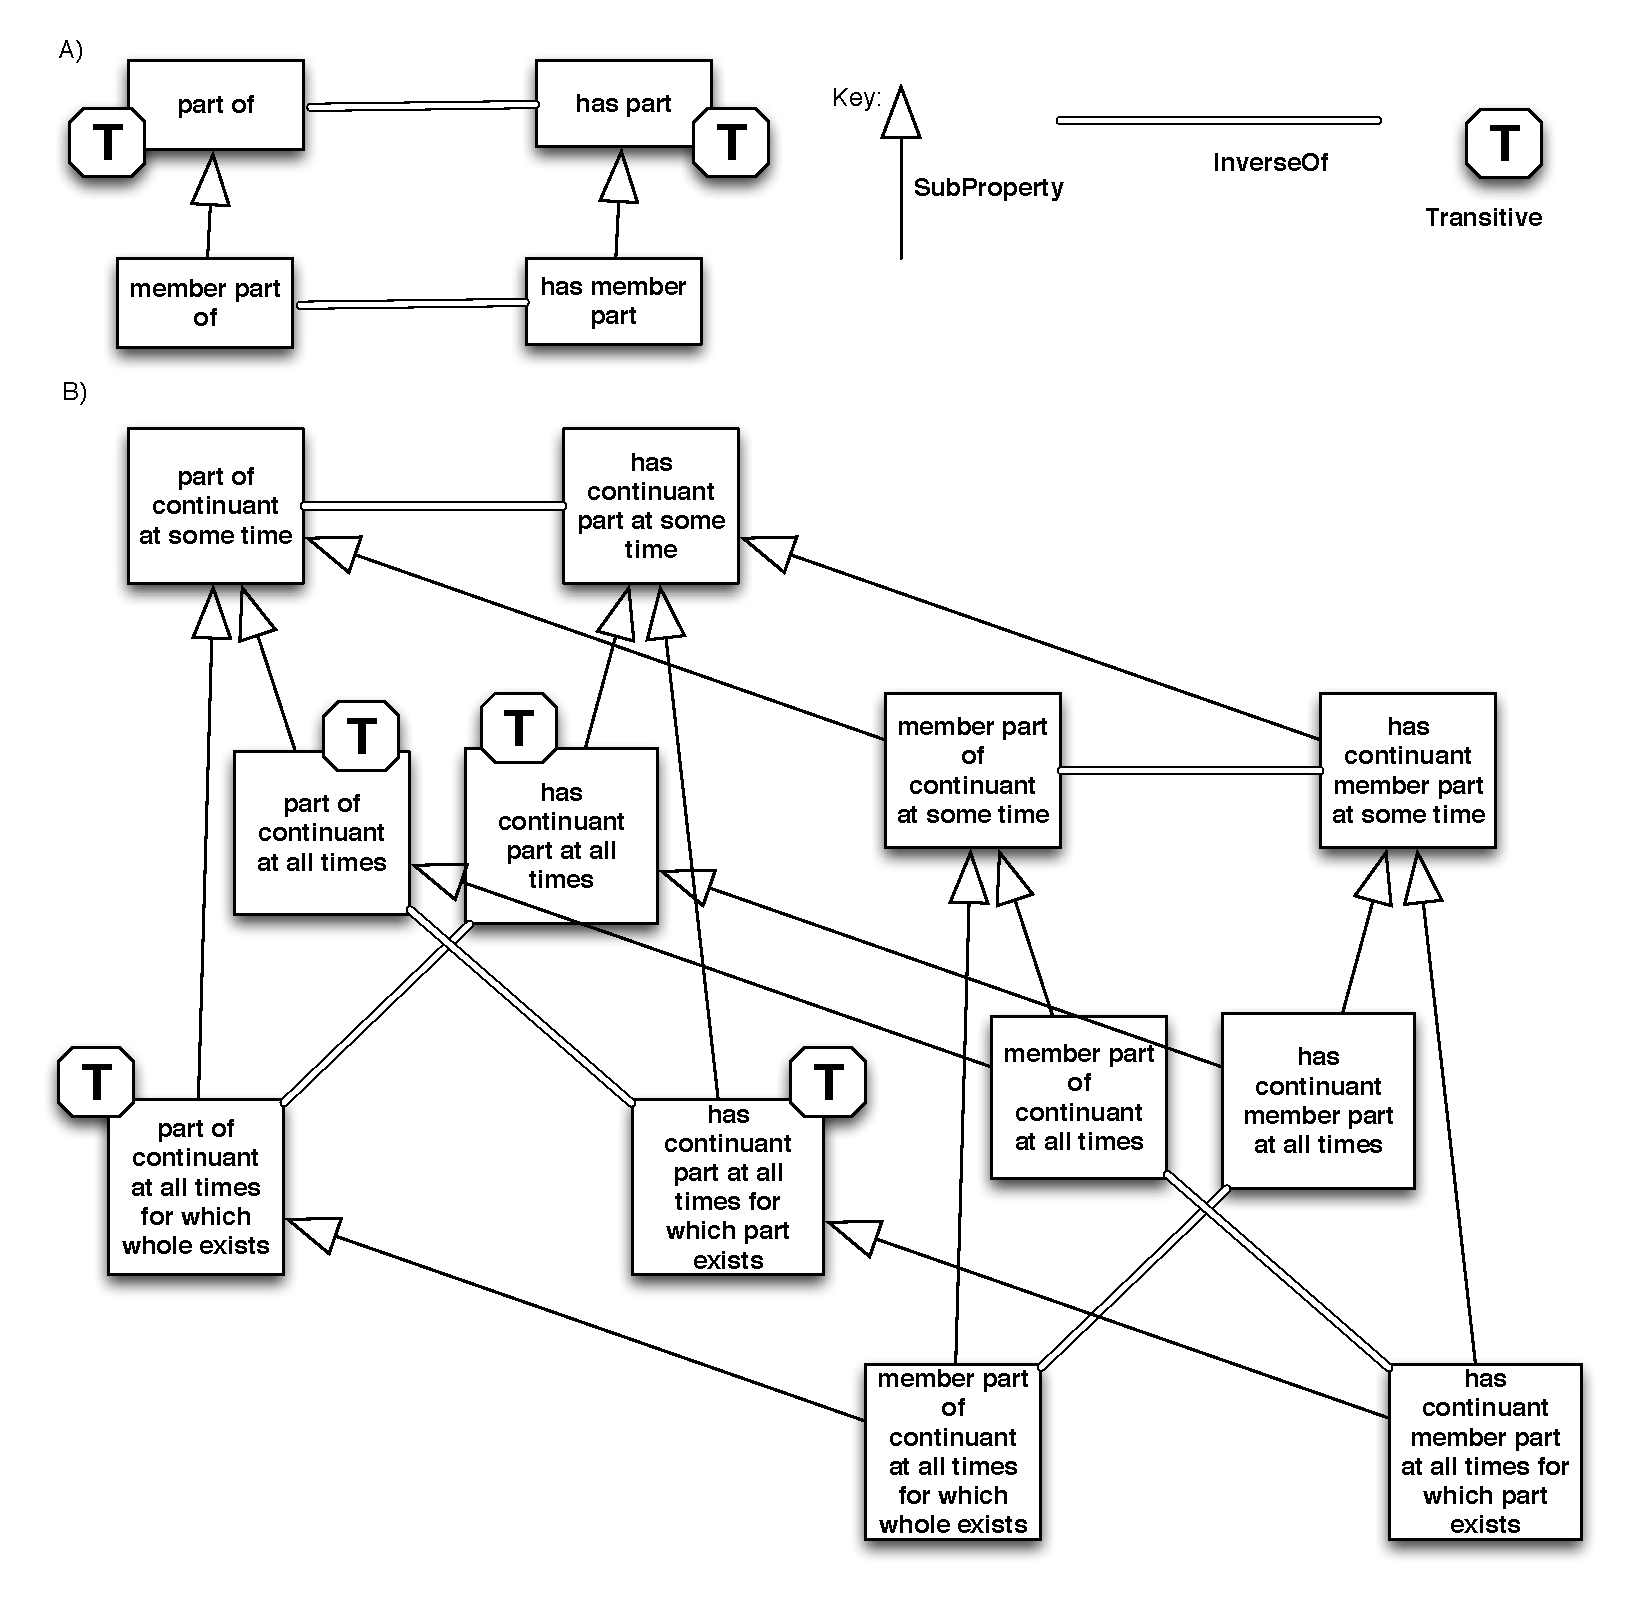
\includegraphics[width=14cm]{member-part}
\caption{Parthood and member-parthood relations, both atemporal (A)
  and temporalized (B). The atemporal form can be found in the current
  RO. The more complex temporalized form can be seen in the BFO2 Graz
  release. As can be seen, the already complex structure found with
  the basic parthood relation is made even more complex with the
  addition of sub-relations.}.
\label{fig:member-part}
\end{figure}
%----------------------------------------


\end{document}
